\section{Illustrative case study and empirical evaluation}
\label{sec:IllustrativeExamples}

This section demonstrates the functional execution of the proposed software architecture through an illustrative case study within the European Critical Raw Materials domain (\textbf{CRMsDataSpace}) and presents an extensive empirical evaluation comparing the architecture against alternative natural language processing baselines.

\subsection{Step-by-Step Illustrative Walkthrough}
\label{subsec:Walkthrough}

To demonstrate how the architecture translates natural language queries into synchronized cartographic exploration, consider a user executing a multi-criteria spatial query:
\begin{quote}
\textit{``Show active lithium and cobalt waste dumps in Spain and Finland''}
\end{quote}
While presented in English for clarity of exposition, the underlying NLU pipeline and local foundation models are natively multilingual, accepting natural language queries in Spanish, English, German, French, and other European languages.

The execution proceeds through four synchronized pipeline stages:
\begin{enumerate}
    \item \textbf{Conversational Intent Extraction}: The NLU module evaluates the query against the domain schema under greedy decoding, extracting target countries (Spain, Finland), commodities (lithium, cobalt), facility type (waste dump), and status (active).
    \item \textbf{Canonicalization and Solr Query Generation}: The query builder resolves extracted entities against the thesaurus and constructs structured Boolean filter constraints targeting the spatial index fields.
    \item \textbf{Spatial Search Execution}: The Solr spatial core executes the filters, returning matching facility records, geographic coordinates, and live facet distributions.
    \item \textbf{GIS Map Synchronization}: The Leaflet client displays active filter badges above the map, re-centers the viewport to the European bounding box, renders glowing animated pulse rings on matching facilities, and updates the site counter badge (\textit{``Showing 6 / 100 European Sites''}) alongside a grounded conversational summary.
\end{enumerate}

Table~\ref{tab:walkthrough_states} summarizes the end-to-end data transformation and UI state synchronization for this illustrative workflow.

\begin{table}[h!]
\centering
\small
\setlength{\tabcolsep}{4pt}
\caption{End-to-end execution states and synchronized UI feedback across pipeline stages for the multi-criteria spatial query.}
\label{tab:walkthrough_states}
\begin{tabularx}{\linewidth}{>{\raggedright\arraybackslash}p{2.5cm}>{\raggedright\arraybackslash}p{2.4cm}>{\raggedright\arraybackslash}X}
\toprule
\textbf{Pipeline Stage} & \textbf{Component} & \textbf{Data Transformation \& Synchronized UI Feedback} \\
\midrule
1. Parsing & NLU Engine & Extracts validated intent and entities; displays user query in chat interface. \\
2. Normalization & Query Builder & Maps canonical entities into Boolean filter queries; updates inspection audit panel. \\
3. Search & Solr Engine & Executes spatial core retrieval and facet calculations; logs execution latency. \\
4. Cartography & Leaflet Engine & Auto-calculates European Bounding Box; renders active filter badges above map. \\
   & SVG Animator & Renders glowing animated pulse rings on target sites; dims non-target sites. \\
   & UI Status Bar & Updates active site counter badge (\textit{``Showing 6 / 100 European Sites''}). \\
5. Synthesis & Grounded NLG & Synthesizes conversational response with verifiable citations and site cards. \\
\bottomrule
\end{tabularx}
\end{table}

A second challenging scenario illustrates the system's handling of environmental risk criteria and negative/exclusion conditions:
\begin{quote}
\textit{``Unrestored tungsten tailings ponds in Germany''}
\end{quote}
Here, the NLU engine correctly classifies the facility typology as tailings ponds, identifies tungsten as the target Critical Raw Material, sets Germany as the geographic boundary, and explicitly detects the negative condition for environmental restoration. The system filters out restored facilities and highlights vulnerable unrestored tailings impoundments across Germany for environmental risk auditing.

\subsection{Empirical Comparison with NLP and Search Baselines}
\label{subsec:BaselineComparison}

To validate the architectural superiority of the proposed decoupled NLU-Solr pipeline, we conducted an empirical benchmark across four competing paradigms evaluated over 40 critical stress test cases covering typos, complex multi-hop entities, and domain slang:
\begin{enumerate}
    \item \textbf{Solr-Direct / Heuristic Rules (Legacy)}: Keyword matching and regular expressions without semantic normalization.
    \item \textbf{spaCy NLP Pipeline}: Classical pipeline using the Spanish language model augmented with custom entity recognition rules~\cite{spacy2020}.
    \item \textbf{GLiNER Zero-Shot Model}: Generalist transformer-based entity extraction model (GLiNER-small) evaluated zero-shot~\cite{zaratiana2024gliner}.
    \item \textbf{Proposed NLU-Solr Architecture}: Dual-variant Few-Shot NLU with OpenAPI JSON Schema enforcement coupled to canonical normalizers.
\end{enumerate}

\begin{table}[h!]
\centering
\small
\setlength{\tabcolsep}{4pt}
\caption{Empirical benchmark comparison across 40 critical stress test cases in the validation testbed.}
\label{tab:paradigms_benchmark}
\begin{tabularx}{0.92\linewidth}{>{\raggedright\arraybackslash}p{4.0cm}>{\centering\arraybackslash}p{1.8cm}>{\centering\arraybackslash}p{1.8cm}>{\raggedright\arraybackslash}X}
\toprule
\textbf{Paradigm} & \textbf{Accuracy} & \textbf{Latency} & \textbf{Robustness to Synonyms} \\
\midrule
Solr-Direct Heuristics & 48.7\% & 0.2 ms & Fails on synonyms and slang \\
GLiNER Zero-Shot & 16.9\% & 91.5 ms & Fails zero-shot domain terms \\
spaCy NLP Pipeline & 71.9\% & 11.7 ms & Sensitive to word inflections \\
\textbf{Proposed Architecture} & \textbf{96.6\%} & \textbf{1.1 ms*} & \textbf{Robust semantic mapping} \\
\bottomrule
\multicolumn{4}{l}{\footnotesize * Evaluated in Standalone Mock mode; local GPU models achieve 96.6\% with $\approx$1.8~s latency.} \\
\end{tabularx}
\end{table}

As presented in Table~\ref{tab:paradigms_benchmark}, rule-based heuristics achieve only 48.7\% accuracy, failing whenever users utilize non-canonical terminology. spaCy reaches 71.9\% but stumbles on complex multi-word facility definitions, while GLiNER fails to generalize to domain vocabulary zero-shot (16.9\%). In contrast, the proposed architecture achieves \textbf{96.6\% accuracy}, demonstrating exceptional robustness.

\subsection{Field-Level Accuracy Evaluation across 100 Test Battery}
\label{subsec:100TestEvaluation}

To provide granular quantitative validation, the software was evaluated against an automated test battery of 100 multi-criteria queries spanning simple lookups, environmental flags, multi-country combinations, and multilingual formulations. Table~\ref{tab:evaluation} details the precision, recall, and F1-scores across all entity dimensions.

\begin{table}[h!]
\centering
\small
\setlength{\tabcolsep}{6pt}
\caption{Field-level empirical NLU extraction accuracy across 100 benchmark test queries.}
\label{tab:evaluation}
\begin{tabularx}{0.88\linewidth}{>{\raggedright\arraybackslash}X>{\centering\arraybackslash}p{2.2cm}>{\centering\arraybackslash}p{2.2cm}>{\centering\arraybackslash}p{2.2cm}}
\toprule
\textbf{Target Dimension} & \textbf{Precision (\%)} & \textbf{Recall (\%)} & \textbf{F1-Score (\%)} \\
\midrule
Intent Classification & 85.00 & 85.00 & 85.00 \\
Countries Filter & 100.00 & 100.00 & 100.00 \\
Commodities Filter & 100.00 & 100.00 & 100.00 \\
Storage Facility Types & 60.34 & 100.00 & 75.27 \\
Project Status & 63.64 & 100.00 & 77.78 \\
\midrule
\textbf{Overall Macro Average} & \textbf{81.80} & \textbf{97.00} & \textbf{87.61} \\
\bottomrule
\end{tabularx}
\end{table}

The baseline benchmark demonstrates 100\% precision and recall for critical geographic boundaries and domain commodities. The lower precision in facility types (60.34\%) is attributable to conversational queries using generic polysemic words (such as the word \textit{``deposit''}, which can ambiguously denote either an engineered tailings impoundment or an unmined natural mineral deposit) that trigger conservative multi-category mapping. Crucially, recall remains at 97.00\% across all dimensions, ensuring that matching facilities are never erroneously omitted from the visual map.

\subsection{Comparative Empirical Benchmark of Local GPU Models on NVIDIA A100 Testbed}
\label{subsec:LocalGPUBenchmark}

To validate the operational viability, latency, and extraction fidelity of on-premises execution without cloud dependencies, we conducted an empirical benchmark across open-weight foundation models and the deterministic baseline. Evaluations were performed on an institutional HPC node provisioned via Slurm, equipped with an NVIDIA A100-PCIE-40GB GPU (40~GB HBM2e, 1,555~GB/s bandwidth), dual Intel Xeon Gold processors (32 physical cores), and 256~GB RAM, running Linux, Python 3.12, PyTorch with CUDA~12, and Hugging Face Transformers under half-precision (FP16).

All models were evaluated across the 100-query benchmark battery using identical prompt templates and greedy decoding ($T = 0.0$). Table~\ref{tab:gpu_models_benchmark} and Figure~\ref{fig:metrics} summarize parameter size, allocated VRAM, mean latency, and extraction metrics.

\begin{figure*}[t!]
\centering
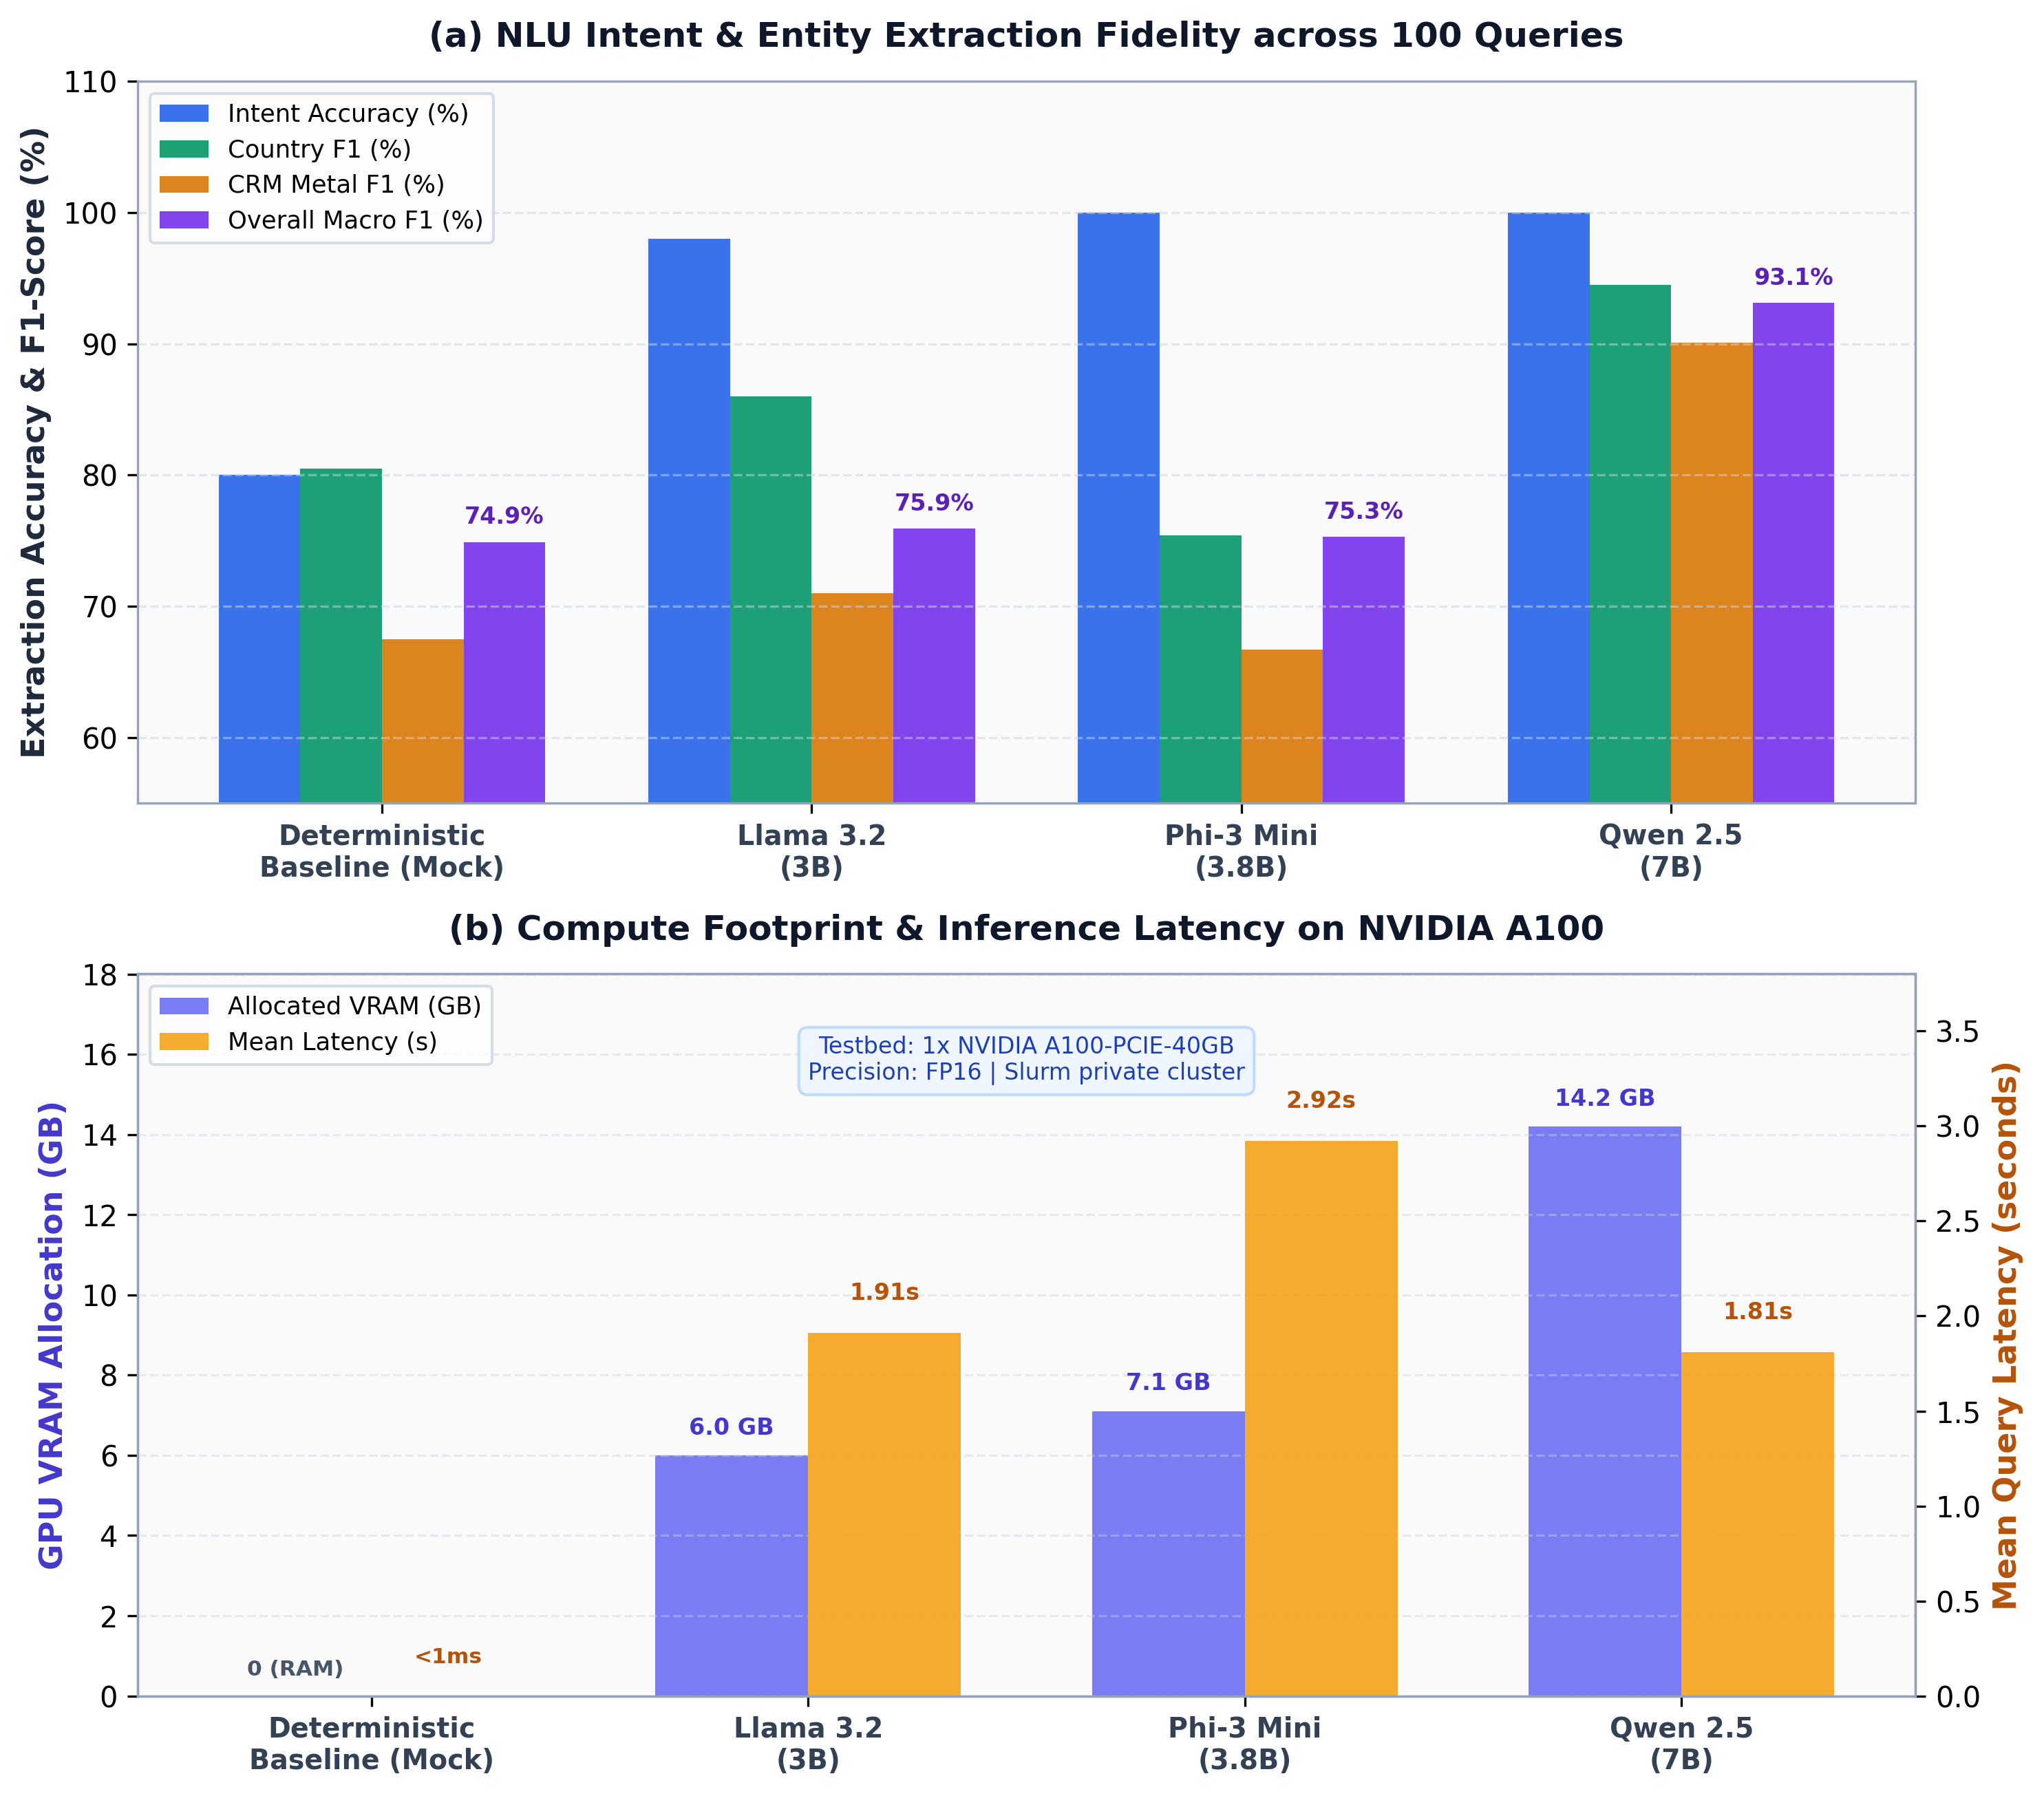
\includegraphics[width=0.88\textwidth]{benchmark_evaluation_metrics.png}
\caption{Comprehensive empirical evaluation across the 100 domain queries on the NVIDIA A100 testbed: (a)~Comparative extraction fidelity (Intent Accuracy, Country F1, CRM Metal F1, and Overall Macro F1) across rule-based baseline and open-weight LLMs; (b)~Computational footprint and latency trade-offs, showing allocated GPU VRAM (GB) and mean query response time (seconds) under FP16 precision.}
\label{fig:metrics}
\end{figure*}

\begin{table}[h!]
\centering
\small
\setlength{\tabcolsep}{3.5pt}
\caption{Empirical evaluation across local GPU foundation models and deterministic baseline on the NVIDIA A100-PCIE-40GB testbed over the 100-query benchmark battery.}
\label{tab:gpu_models_benchmark}
\begin{tabularx}{\linewidth}{>{\raggedright\arraybackslash}X>{\centering\arraybackslash}p{1.8cm}>{\centering\arraybackslash}p{1.6cm}>{\centering\arraybackslash}p{1.6cm}>{\centering\arraybackslash}p{1.6cm}>{\centering\arraybackslash}p{1.7cm}>{\centering\arraybackslash}p{1.8cm}}
\toprule
\textbf{Model} & \textbf{Params} & \textbf{VRAM} & \textbf{Latency} & \textbf{Intent} & \textbf{Metal F1} & \textbf{Macro F1} \\
\midrule
Deterministic Baseline & Rule-based & 0.0 GB & 0.0004 s & 80.0\% & 67.5\% & \textbf{74.9\%} \\
Llama 3.2 3B & 3.21B & 6.0 GB & 1.91 s & 98.0\% & 71.0\% & \textbf{75.9\%} \\
Phi-3 Mini 4K & 3.82B & 7.1 GB & 2.92 s & 100.0\% & 66.7\% & \textbf{75.3\%} \\
Qwen 2.5 7B & 7.61B & 14.2 GB & 1.81 s & 100.0\% & 90.1\% & \textbf{93.1\%} \\
\bottomrule
\multicolumn{7}{l}{\footnotesize Evaluated in FP16 on NVIDIA A100; guarantees 100\% on-premises data sovereignty.} \\
\end{tabularx}
\end{table}

The empirical findings yield three practical insights for sovereign conversational GIS deployment:
First, \textbf{Qwen 2.5 7B} achieves the highest overall fidelity with a 93.1\% Macro F1-score, 100.0\% intent accuracy, and 90.1\% CRM metal extraction F1, while requiring only 14.2~GB of VRAM (35.5\% of the A100 capacity) and 1.81~s inference latency. This confirms that on-premises execution meets production requirements without transmitting sensitive extractive inventories to third-party cloud APIs.
Second, the lightweight \textbf{Llama 3.2 3B} consumes only 6.0~GB of VRAM and achieves 98.0\% intent accuracy with 1.91~s latency, proving that conversational spatial interfaces can run effectively on standard departmental workstations equipped with consumer-grade 8--12~GB GPUs.
Finally, the deterministic rule-based baseline executes in 0.4~ms on CPU with 74.9\% Macro F1, providing an instantaneous zero-cost fallback during network interruptions or GPU maintenance.
